\documentclass[10pt,conference,twocolumn]{IEEEtran}
\IEEEoverridecommandlockouts
\usepackage{cite}
\usepackage{amsmath,amssymb,amsfonts}
\usepackage{graphicx}
\usepackage{booktabs}
\usepackage{stfloats}
\usepackage{pifont}
\usepackage{xcolor}
\usepackage{hyperref}

\hypersetup{
    colorlinks=true,
    linkcolor=blue,
    citecolor=blue,
    urlcolor=blue
}

% Conteúdo novo/atualizado em relação ao Draft anterior destacado em vermelho.
% Para gerar uma versão final toda em preto, basta descomentar a linha abaixo:
\newcommand{\novo}[1]{\textcolor{red}{#1}}
% \renewcommand{\novo}[1]{#1}

\begin{document}

\title{Validade Temporal e Supersessão de Fatos em Memória Associativa Hebbiana para Agentes Baseados em LLM}

\author{\IEEEauthorblockN{Filipe Augusto de Ataíde Barbosa}
\IEEEauthorblockA{\textit{Centro de Informática (CIn) --- Universidade Federal de Pernambuco (UFPE)}\\
Recife, Brasil --- faab@cin.ufpe.br}
}

\maketitle

\begin{abstract}
Memórias associativas hebbianas como o \textit{HeLa-Mem} (ACL 2026) tratam fatos semânticos extraídos como estáticos, sem distinguir quando um fato foi registrado de quando ele deixou de ser verdadeiro. Este trabalho estende a memória semântica do \textit{HeLa-Mem} com janelas explícitas de validade $[t_{start}, t_{end}]$, supersessão não-destrutiva (\texttt{SUPERSEDES}), pertinência temporal $\mathcal{V}(f_i, t_{query})$ e sinalização de vigência no prompt. Avaliado nas 500 questões do \textit{LongMemEval} distribuídas com o código oficial (variante \textit{oracle}, apenas sessões de evidência), \novo{o estudo restaura primeiro uma Baseline Fiel ($A^*$, 100\% dos grafos íntegros e parâmetros oficiais: 63,40\% global e \textit{Multi-Session} em 57,14\%, idêntico ao artigo)} e avalia uma ablação controlada ($B_0$, extração por sessão sem mecanismo temporal, 64,20\%). A Proposta $B$ alcança 65,60\% global e eleva \textit{Knowledge Update} de \novo{67,95\% ($A^*$) e} 65,38\% ($B_0$) para 83,33\% (\novo{+12 acertos sobre $A^*$, McNemar bilateral $p = 0{,}0042$;} +14/$-$0 sobre $B_0$, $p_{\text{Holm}} = 0{,}0015$), \novo{muito acima do piso de ruído medido em réplica independente $B'$ (97,44\% de estabilidade em KU). Uma ablação fatorial 2$\times$2 desacopla os subcomponentes e revela que, no regime \textit{oracle}, as etiquetas de vigência (\texttt{tags\_only}: 66,20\% global; 85,90\% em KU, +16/$-$0) explicam integralmente o ganho, enquanto o re-ranking isolado por $\mathcal{V}$ (\texttt{score\_only}) tem efeito nulo em KU (65,38\%). Uma variante ontológica sem exemplos de domínio ($B_{\text{v2}}$, baseada em \textit{Event Calculus}) corta as supersessões em 53,6\%, eleva a precisão auditada do classificador de 33,3\% para 48,9\% e atinge 57,89\% em \textit{Temporal Reasoning} mantendo significância em KU (79,49\%, $p = 0{,}0117$ vs.\ $A^*$). A análise de sensibilidade em $\lambda \in \{0{,}4; 0{,}6; 0{,}8\}$ e $\tau \in \{30, 60, 90\}$ dias confirma robustez (amplitude global de 1,20 p.p.; KU entre 79,49\% e 84,62\%).}
\end{abstract}

\begin{IEEEkeywords}
Memória para Agentes, Aprendizado Hebbiano, Validade Temporal, Supersessão Factual, \novo{Event Calculus,} LongMemEval.
\end{IEEEkeywords}

\begin{figure*}[!t]
\centering
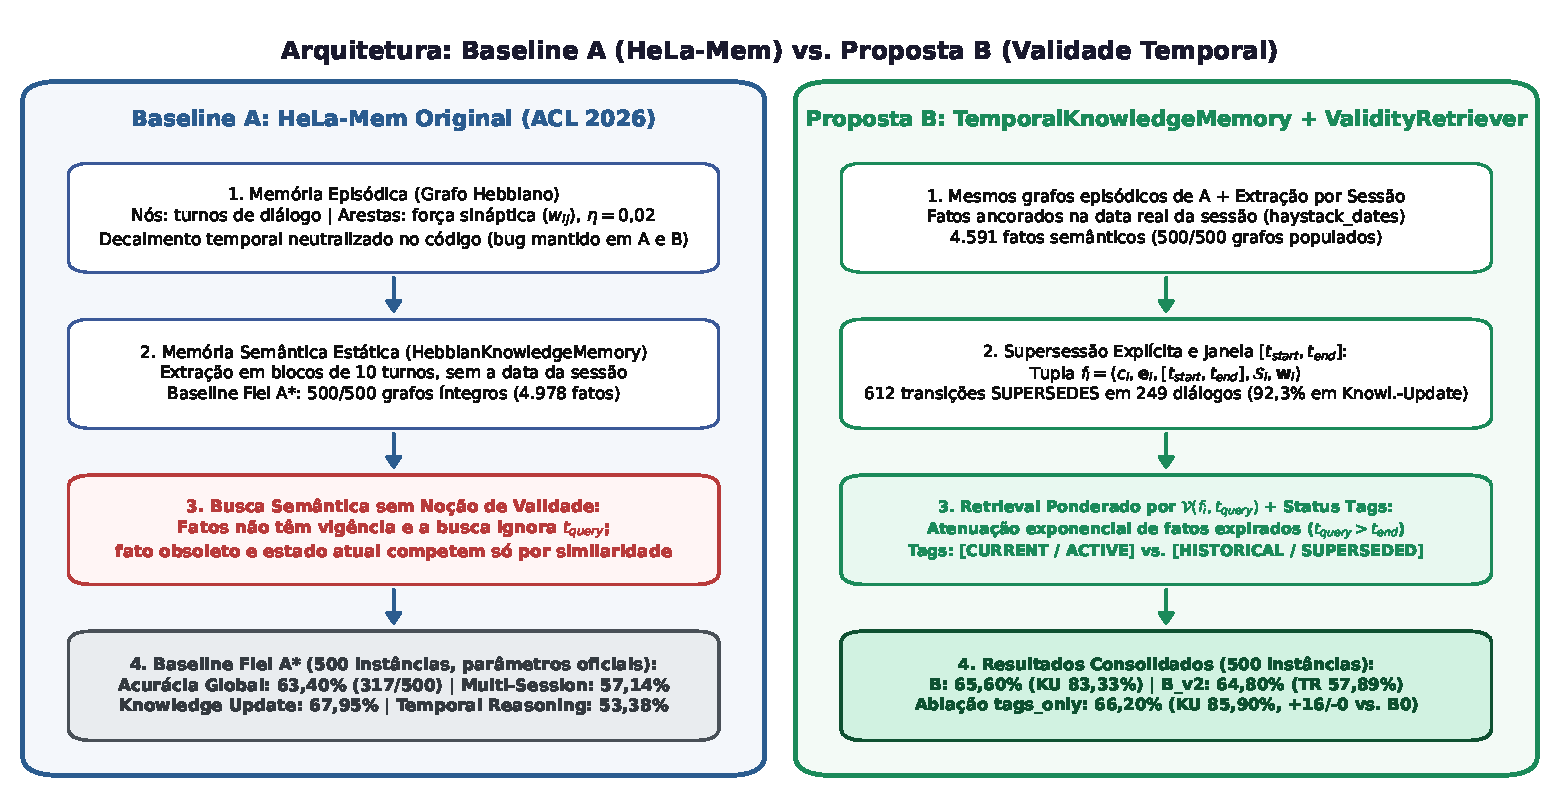
\includegraphics[width=\textwidth]{figures/fig1_arquitetura_proposta.pdf}
\caption{Arquitetura comparada. (Esquerda) \novo{Baseline Fiel $A^*$ (\textit{HeLa-Mem} original com parâmetros oficiais e 500/500 grafos íntegros, 63,40\% global):} memória semântica sem vigência dos fatos e busca que ignora $t_{query}$. (Direita) Proposta Temporal ($B$ \novo{/ $B_{\text{v2}}$}): extração ancorada na data da sessão, janelas de validade $[t_{start}, t_{end}]$, arestas \texttt{SUPERSEDES}, busca ponderada por $\mathcal{V}(f_i, t_{query})$ e etiquetas \texttt{[CURRENT]} / \texttt{[HISTORICAL]} no prompt.}
\label{fig:arquitetura}
\end{figure*}

% =========================================================================
% SEÇÃO I: INTRODUÇÃO
% =========================================================================
\section{Introdução}
Agentes baseados em LLM precisam reter informações ao longo de muitas sessões, e parte dessas informações muda: um endereço, um limite financeiro, uma preferência ativa ou o responsável por um projeto. Uma memória que apenas acumula fatos sem modelo de vigência tende a recuperar estados obsoletos quando eles possuem alta similaridade lexical com a consulta. O \textit{HeLa-Mem}~\cite{helamem2026} organiza a memória em um grafo ponderado com aprendizado hebbiano e ativação espalhada (\textit{spreading activation}), mas não modela durante qual intervalo um fato permaneceu verdadeiro.

Inspirado em grafos de conhecimento temporais (\textit{Zep/Graphiti})~\cite{zep2025}, este trabalho investiga a seguinte pergunta de pesquisa: \textit{a representação explícita da validade temporal e da supersessão de fatos melhora uma memória associativa hebbiana em tarefas de atualização de conhecimento e raciocínio temporal, quando comparada ao mecanismo original?} Seguindo rigorosamente a metodologia experimental da disciplina, o \textit{HeLa-Mem} foi primeiro reproduzido sem modificações, \novo{diagnosticado e restaurado em uma Baseline Fiel ($A^*$), e então comparado de forma controlada contra a extensão temporal ($B$ e variante ontológica $B_{\text{v2}}$), ablações fatoriais ($B_0$, \texttt{score\_only}, \texttt{tags\_only}), réplica de ruído estocástico ($B'$) e análise de sensibilidade ($\lambda, \tau$).}

% =========================================================================
% SEÇÃO II: SOLUÇÃO PROPOSTA
% =========================================================================
\section{Solução Proposta}

\subsection{Diagnóstico do Código Oficial do HeLa-Mem}
No \textit{HeLa-Mem}~\cite{helamem2026}, conexões entre nós episódicos coativados são fortalecidas por aprendizado hebbiano ($\Delta w_{ij} = \eta$), favorecendo a recuperação \textit{multi-hop}. A inspeção do código oficial (\texttt{commit 68f19b3}) revelou três limitações estruturais para o tratamento de fatos mutáveis:
\begin{enumerate}
    \item \textbf{Atemporalidade Semântica}: fatos em \texttt{HebbianKnowledgeMemory} recebem apenas o metadado estático \texttt{\{"type": "fact"\}} e o horário de execução do script (\texttt{get\_timestamp()}) em vez da data real da sessão (\texttt{haystack\_dates}).
    \item \textbf{Competição entre Fatos Conflitantes}: quando um atributo do usuário é atualizado, o fato obsoleto e o atual coexistem em pé de igualdade, competindo apenas por similaridade vetorial.
    \item \textbf{Decaimento Neutralizado e Omissão de $t_{query}$}: em \texttt{hebbian\_memory.py}, a chamada \texttt{compute\_time\_decay(node["timestamp"], current\_time)} passa uma string de data no lugar do escalar $\tau$, caindo silenciosamente em \texttt{except: return 1.0}. Ademais, \texttt{question\_date} é enviada ao prompt final, mas ignorada na etapa de \textit{retrieval}.
\end{enumerate}

\subsection{Formalização, Supersessão \texorpdfstring{\novo{e Classificador Ontológico ($B_{\text{v2}}$)}}{e Classificador Ontológico (B\_v2)}}
A extensão implementada (\texttt{TemporalKnowledgeMemory}) preserva intacto o grafo episódico hebbiano e reformula a memória semântica (Fig.~\ref{fig:arquitetura}). Cada fato $f_i \in \mathcal{F}$ é representado pela 5-upla:
\begin{equation}
f_i = \langle c_i, \mathbf{e}_i, [t_{start}^{(i)}, t_{end}^{(i)}], \mathcal{S}_i, \mathbf{w}_i \rangle
\end{equation}
onde $c_i$ é o conteúdo textual, $\mathbf{e}_i \in \mathbb{R}^d$ o embedding normalizado, $[t_{start}^{(i)}, t_{end}^{(i)}]$ a janela de validade ancorada na data da sessão ($t_{end}^{(i)} = \infty$ enquanto ativo), $\mathcal{S}_i$ os ponteiros de supersessão (\texttt{superseded\_by}/\texttt{supersedes}) e $\mathbf{w}_i$ os pesos hebbianos.

Ao extrair um novo fato $f_{new}$ de uma sessão em $t_{event}$, selecionam-se candidatos ativos de sessões anteriores ($\mathcal{F}_{active} = \{f_{cand} \mid t_{end}^{(cand)} = \infty \land t_{start}^{(cand)} \neq t_{event}\}$) com $\mathbf{e}_{new}^\top \mathbf{e}_{cand} \ge \theta_{sup}$ ($\theta_{sup} = 0{,}35$). Os 4 candidatos mais similares são classificados por um LLM em três estados:
\begin{itemize}
    \item \textbf{UNRELATED}: entidades ou tópicos independentes; ambos permanecem ativos.
    \item \textbf{EXTENDS}: $f_{new}$ complementa $f_{cand}$ sem contradição; reforça-se $w(f_{cand}, f_{new}) \leftarrow w(f_{cand}, f_{new}) + \eta$.
    \item \textbf{SUPERSEDES}: $f_{new}$ substitui o estado descrito em $f_{cand}$, encerrando sua vigência de forma não-destrutiva:
    \begin{align}
    t_{end}^{(cand)} &\leftarrow t_{event}, \quad \mathcal{S}_{cand} \leftarrow f_{new}, \nonumber \\
    [t_{start}^{(new)}, t_{end}^{(new)}] &\leftarrow [t_{event}, \infty)
    \end{align}
    criando uma aresta bidirecional de peso $w = 0{,}8$ entre $f_{cand}$ e $f_{new}$ para preservar a linhagem histórica.
\end{itemize}

\novo{Após observar \textit{over-supersession} em tarefas de contagem na formulação inicial ($B$), desenvolveu-se a variante ontológica \textbf{$B_{\text{v2}}$}, que remove todos os exemplos de domínio do prompt do classificador (eliminando risco de viés de indução por prompt) e fundamenta a decisão exclusivamente em \textit{Event Calculus}: \texttt{SUPERSEDES} restringe-se a atributos unívocos ou estados mutuamente exclusivos de uma entidade, enquanto \texttt{EXTENDS} abrange eventos históricos independentes, transações e entidades coexistentes.}

\begin{figure*}[!t]
\centering
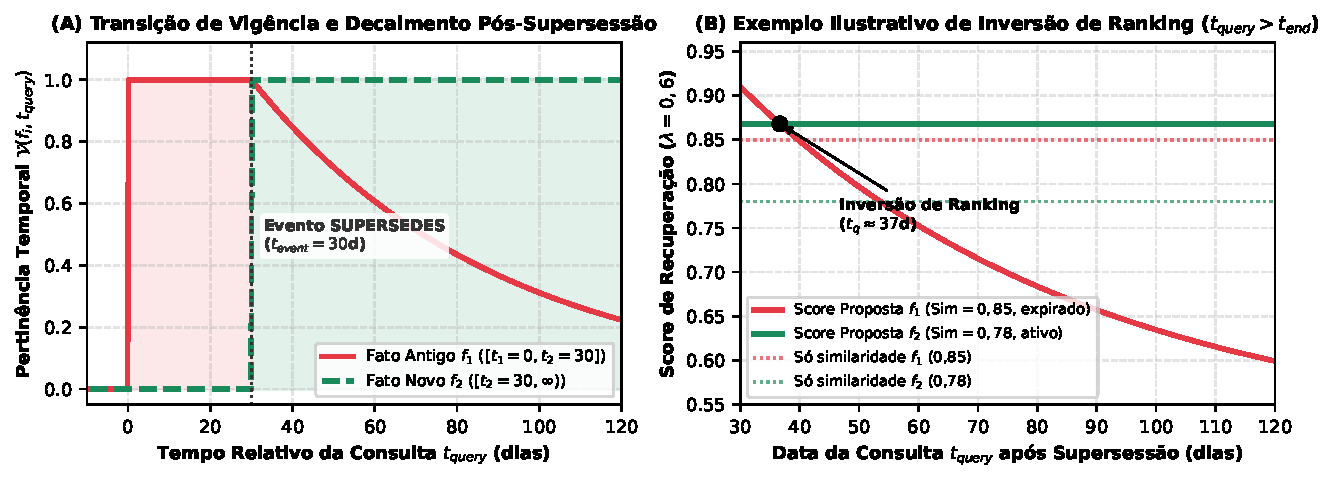
\includegraphics[width=0.92\textwidth]{figures/fig5_decaimento_pertinencia.pdf}
\caption{Comportamento analítico da pertinência temporal $\mathcal{V}(f_i, t_{query})$: (A) fechamento da vigência de $f_1$ na supersessão ($t_{event}=30$\,d) e atenuação exponencial ($\tau_{decay}=60$\,d); (B) inversão de ranking sob $\lambda=0{,}6$ quando o fato obsoleto $f_1$ possui maior similaridade lexical ($\widetilde{\text{Sim}}=0{,}85$) do que o fato vigente $f_2$ ($\widetilde{\text{Sim}}=0{,}78$).}
\label{fig:decaimento}
\end{figure*}

\subsection{Retrieval Ponderado por $\mathcal{V}(f_i, t_{query})$ e Etiquetas no Prompt}
Na consulta $Q$ em $t_{query}$, o módulo \texttt{ValidityAwareRetriever} calcula a pertinência temporal de cada fato:
\begin{equation}
\mathcal{V}(f_i, t_{query}) =
\begin{cases}
1, & \text{se } t_{start}^{(i)} \le t_{query} \le t_{end}^{(i)} \\
\exp\left(-\frac{t_{query} - t_{end}^{(i)}}{\tau_{decay}}\right), & \text{se } t_{query} > t_{end}^{(i)} \\
0, & \text{se } t_{query} < t_{start}^{(i)}
\end{cases}
\end{equation}
e combina similaridade reescalada $\widetilde{\text{Sim}}(\mathbf{e}_i, \mathbf{e}_Q) = (\mathbf{e}_i^\top \mathbf{e}_Q + 1)/2$ com $\mathcal{V}$ ($\lambda = 0{,}6$, $\tau_{decay} = 60$\,d) antes da ativação espalhada:
\begin{equation}
\text{Score}(f_i, Q, t_{query}) = \lambda \, \widetilde{\text{Sim}}(\mathbf{e}_i, \mathbf{e}_Q) + (1-\lambda) \, \mathcal{V}(f_i, t_{query}) + \text{Spread}(f_i)
\end{equation}
Os fatos recuperados são formatados no bloco \texttt{<KNOWLEDGE BASE>} com etiquetas explícitas: \texttt{[CURRENT / ACTIVE (Valid since: $t_{start}$)]} ou \texttt{[HISTORICAL / SUPERSEDED (Valid: $t_{start}$ to $t_{end}$)]}.

% =========================================================================
% SEÇÃO III: PROTOCOLO EXPERIMENTAL
% =========================================================================
\section{Protocolo Experimental}

\begin{itemize}
    \item \textbf{Dataset e recorte \textit{oracle}}: 500 questões do arquivo \texttt{data/longmemeval\_s.json} distribuído no repositório oficial do \textit{HeLa-Mem}~\cite{longmemeval2025}, em 6 categorias. A auditoria verificou que esse arquivo contém \textbf{apenas as sessões de evidência} (1 a 6 sessões; média de 1,0 nas categorias de sessão única e 2,0--2,6 nas demais), correspondendo à variante \textit{oracle} e não às $\sim$40 sessões ($\sim$115k tokens) do \textit{LongMemEval\textsubscript{S}} oficial. \novo{Confirmou-se que os baselines externos da Tabela 6 do artigo-base provêm do \textit{LightMem} no split completo de $\sim$115k tokens; por transparência metodológica, todas as conclusões deste estudo baseiam-se exclusivamente em comparações internas pareadas sobre o mesmo arquivo.}
    \item \novo{\textbf{Diagnóstico da Baseline inicial ($A$) e restauração da Baseline Fiel ($A^*$)}: na primeira reprodução ($A$, 61,20\%), a execução paralela multithreaded no Windows provocou exceções silenciosas engolidas pelo bloco \texttt{try/except} de \texttt{process\_incremental\_buffer}, deixando 360/500 grafos semânticos vazios, além de dois desvios de hiperparâmetro (\texttt{MAX\_FLIPPED}=5 vs.\ 3 e \texttt{KEYWORD\_WEIGHT}=0,5 vs.\ 0,7). Um teste diagnóstico sequencial (\texttt{workers=1}) no item 400 (bloco onde 50/50 estavam vazios) comprovou a falha de concorrência ao extrair 9 nós semânticos nominais. Executou-se então a \textbf{Baseline Fiel ($A^*$)} com controle estrito de workers (\texttt{workers=2}) e conformidade integral aos scripts oficiais (\texttt{MAX\_FLIPPED}=3, \texttt{KEYWORD\_WEIGHT}=0,7, \texttt{TOP\_K}=15, \texttt{BUFFER\_SIZE}=10), atingindo \textbf{500/500 grafos íntegros} (4.978 nós semânticos).}
    \item \textbf{Desenho pareado e ablações}: todas as condições usam \texttt{gpt-4o-mini} (extração, geração e juiz LLM oficial do \textit{LongMemEval}, \texttt{temperature}=0,7) e \texttt{all-MiniLM-L6-v2}. Sobre exatamente os mesmos 500 grafos codificados da Proposta $B$ (4.591 fatos extraídos por sessão), avaliaram-se: (i) \textbf{$B_0$} (\texttt{no\_temporal}: sem validade, sem arestas do classificador, prompt original); \novo{(ii) \textbf{\texttt{score\_only}} ($\mathcal{V}$ ligado, sem etiquetas no prompt); (iii) \textbf{\texttt{tags\_only}} ($\mathcal{V}\equiv 1$, etiquetas ligadas); (iv) \textbf{$B'$} (réplica independente completa para medir o piso de ruído estocástico); e (v) análise de sensibilidade pré-registrada em $\lambda \in \{0{,}4; 0{,}8\}$ e $\tau \in \{30\text{d}, 90\text{d}\}$ sem seleção de hiperparâmetros no conjunto de teste.}
\end{itemize}

% =========================================================================
% SEÇÃO IV: RESULTADOS E ANÁLISE QUANTITATIVA
% =========================================================================
\section{Resultados e Análise Quantitativa}

\subsection{Trajetória Completa e Desempenho por Categoria}
A Tabela~\ref{tab:evolucao} resume todas as condições avaliadas nas 500 questões, e a Tabela~\ref{tab:ab_results} (ilustrada na Fig.~\ref{fig:baseline_vs_paper}) detalha o desempenho por categoria.

\begin{table}[!t]
\caption{Síntese das condições experimentais avaliadas ($N = 500$). \novo{Novas condições em vermelho.}}
\label{tab:evolucao}
\centering
\footnotesize
\setlength{\tabcolsep}{3.2pt}
\begin{tabular}{lccp{2.6cm}}
\toprule
\textbf{Condição} & \textbf{Global} & \textbf{KU (78)} & \textbf{Papel experimental} \\
\midrule
Baseline $A$ (inicial) & 61,20\% & 57 (73,08\%) & \novo{360 grafos vazios (concorrência)} \\
\novo{\textbf{Baseline Fiel $A^*$}} & \novo{\textbf{63,40\%}} & \novo{\textbf{53 (67,95\%)}} & \novo{\textbf{0 vazios; parâmetros oficiais}} \\
Ablação $B_0$ & 64,20\% & 51 (65,38\%) & extração/sessão, sem tempo \\
\novo{\texttt{score\_only}} & \novo{61,80\%} & \novo{51 (65,38\%)} & \novo{só $\mathcal{V}$, sem etiquetas} \\
\novo{\textbf{\texttt{tags\_only}}} & \novo{\textbf{66,20\%}} & \novo{\textbf{67 (85,90\%)}} & \novo{\textbf{só etiquetas, $\mathcal{V}\equiv 1$}} \\
Proposta $B$ (ref.) & 65,60\% & 65 (83,33\%) & $\mathcal{V}$ + etiquetas ($\lambda=0{,}6, \tau=60$d) \\
\novo{Réplica $B'$} & \novo{64,00\%} & \novo{65 (83,33\%)} & \novo{piso de ruído (97,4\% est.\ KU)} \\
\novo{Proposta $B_{\text{v2}}$} & \novo{64,80\%} & \novo{62 (79,49\%)} & \novo{classificador \textit{Event Calculus}} \\
\bottomrule
\end{tabular}
\end{table}

\begin{table*}[!t]
\caption{Acurácia por categoria nas 500 questões: \novo{Baseline Fiel ($A^*$),} ablação $B_0$, Proposta $B$\novo{, Proposta Ontológica ($B_{\text{v2}}$) e ablação \texttt{tags\_only}}.}
\label{tab:ab_results}
\centering
\footnotesize
\setlength{\tabcolsep}{5.0pt}
\begin{tabular}{lcccccc}
\toprule
\textbf{Categoria (\texttt{question\_type})} & \textbf{$N$} & \novo{\textbf{Baseline Fiel $A^*$}} & \textbf{Ablação $B_0$} & \textbf{Proposta $B$} & \novo{\textbf{Proposta $B_{\text{v2}}$}} & \novo{\textbf{\texttt{tags\_only}}} \\
\midrule
\texttt{knowledge-update} & 78 & \novo{53 (67,95\%)} & 51 (65,38\%) & 65 (83,33\%)$^*$ & \novo{62 (79,49\%)$^*$} & \novo{\textbf{67 (85,90\%)}$^*$} \\
\texttt{temporal-reasoning} & 133 & \novo{71 (53,38\%)} & 76 (57,14\%) & 74 (55,64\%) & \novo{\textbf{77 (57,89\%)}} & \novo{75 (56,39\%)} \\
\texttt{multi-session} & 133 & \novo{\textbf{76 (57,14\%)}} & 72 (54,14\%) & 65 (48,87\%) & \novo{68 (51,13\%)} & \novo{68 (51,13\%)} \\
\texttt{single-session-preference} & 30 & \novo{10 (33,33\%)} & 12 (40,00\%) & \textbf{14 (46,67\%)} & \novo{12 (40,00\%)} & \novo{11 (36,67\%)} \\
\texttt{single-session-assistant} & 56 & \novo{51 (91,07\%)} & 50 (89,29\%) & \textbf{52 (92,86\%)} & \novo{49 (87,50\%)} & \novo{51 (91,07\%)} \\
\texttt{single-session-user} & 70 & \novo{56 (80,00\%)} & \textbf{60 (85,71\%)} & 58 (82,86\%) & \novo{56 (80,00\%)} & \novo{59 (84,29\%)} \\
\midrule
\textbf{OVERALL (Global)} & \textbf{500} & \novo{\textbf{317 (63,40\%)}} & \textbf{321 (64,20\%)} & \textbf{328 (65,60\%)} & \novo{\textbf{324 (64,80\%)}} & \novo{\textbf{331 (66,20\%)}} \\
\bottomrule
\multicolumn{7}{l}{\scriptsize $^*$Significância estatística em \textit{Knowledge Update} (McNemar bilateral): \novo{$A^*\!\rightarrow\!B$ ($p=0{,}0042$), $A^*\!\rightarrow\!B_{\text{v2}}$ ($p=0{,}0117$),} $B_0\!\rightarrow\!B$ ($p_{\text{Holm}}=0{,}0015$)\novo{, $B_0\!\rightarrow\!\texttt{tags\_only}$ ($p<0{,}0001$)}.}
\end{tabular}
\end{table*}

\begin{figure}[!t]
\centering
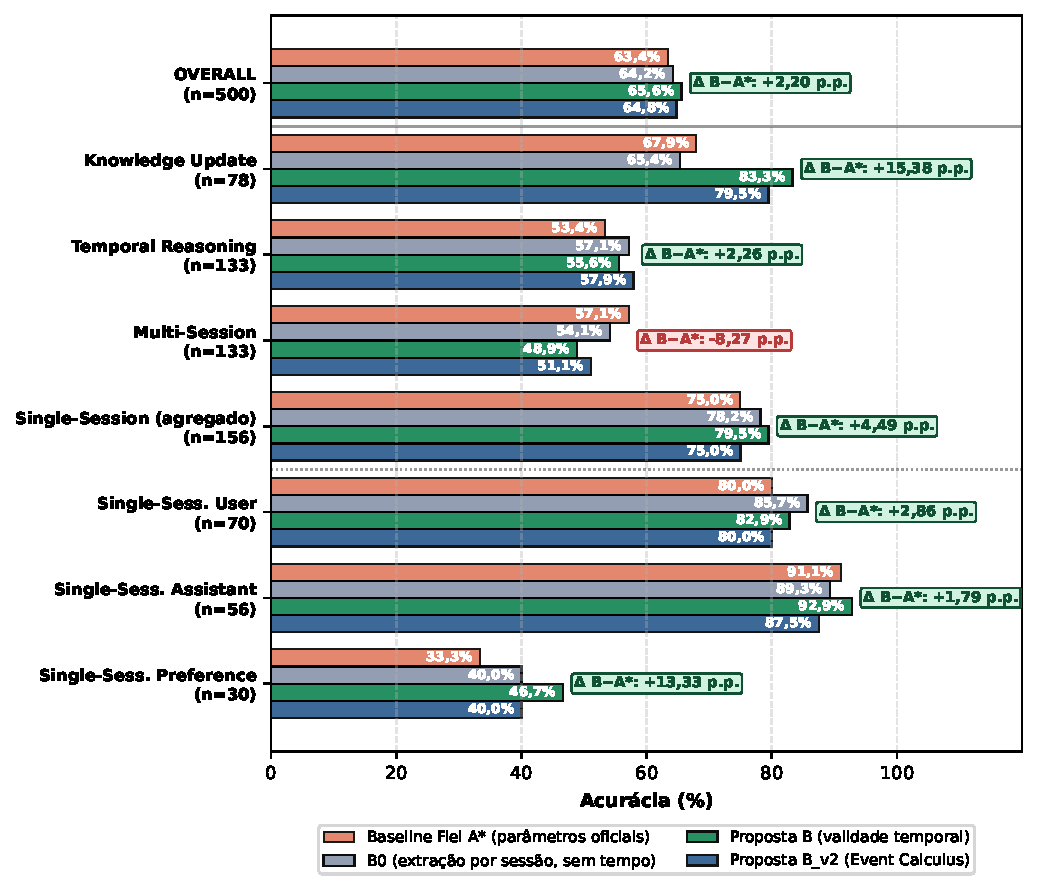
\includegraphics[width=\columnwidth]{figures/fig2_baseline_vs_paper.pdf}
\caption{Acurácia por categoria: \novo{Baseline Fiel ($A^*$),} ablação $B_0$, Proposta $B$ \novo{e Proposta $B_{\text{v2}}$. Os rótulos indicam $\Delta(B - A^*)$ em pontos percentuais.}}
\label{fig:baseline_vs_paper}
\end{figure}

Quatro achados centrais emergem das Tabelas~\ref{tab:evolucao} e~\ref{tab:ab_results}:
\begin{enumerate}
    \item \textbf{\novo{Restauração da Baseline ($A \rightarrow A^*$) e} interferência factual}: \novo{com 100\% dos grafos íntegros e \texttt{KEYWORD\_WEIGHT}=0,7, $A^*$ atingiu exatamente os \textbf{57,14\% (76/133)} reportados no artigo em \textit{Multi-Session}. Em contrapartida, \textit{Knowledge Update} caiu de 73,08\% ($A$) para \textbf{67,95\% ($A^*$)}}, acompanhando a queda já vista em \textbf{65,38\% ($B_0$)}. Isso comprova o \textit{fenômeno da interferência factual}: extrair fatos semânticos densos sem modelar validade temporal injeta asserções obsoletas e vigentes como itens indistinguíveis no prompt, degradando atualizações.
    \item \textbf{Confirmação causal em \textit{Knowledge Update}}: a introdução da validade temporal desfaz essa interferência e eleva KU para \textbf{83,33\%} ($B$: +14/$-$0 sobre $B_0$, $p_{\text{Holm}} = 0{,}0015$\novo{; +12 sobre $A^*$, $p = 0{,}0042$}) \novo{e \textbf{79,49\%} ($B_{\text{v2}}$: +9 sobre $A^*$, $p = 0{,}0117$; +12/$-$1 sobre $B_0$, $p = 0{,}0034$)}.
    \item \novo{\textbf{Mitigação de regressões em $B_{\text{v2}}$}: o classificador ontológico reduziu o volume de supersessões em \textbf{53,6\%} (612 $\rightarrow$ 284), recuperou parte das regressões em \textit{Multi-Session} (de 48,87\% para 51,13\%) e atingiu o maior desempenho do projeto em \textit{Temporal Reasoning} (\textbf{57,89\%}).}
    \item \novo{\textbf{Piso de ruído estocástico ($B \times B'$)}}: \novo{a reavaliação completa $B'$ sob \texttt{temperature}=0,7 registrou 36 pares discordantes no geral (7,20\%, 65,60\% vs.\ 64,00\%, $p = 0{,}243$), mas \textbf{estabilidade de 97,44\% em \textit{Knowledge Update}} (ambas em 83,33\%, apenas +1/$-$1). O ganho causal (+14 sobre $B_0$; +12 sobre $A^*$) supera o ruído em mais de 6 vezes.}
\end{enumerate}

\subsection{Estatística Pareada (McNemar)}
A Tabela~\ref{tab:mcnemar} e a Fig.~\ref{fig:analise_pareada} consolidam os testes exatos de McNemar bilaterais. No agregado global ($N = 500$), os ganhos em \textit{Knowledge Update} são parcialmente contrabalançados pelo custo em \textit{Multi-Session}, fazendo com que \novo{$A^* \rightarrow B$ (+11, $p = 0{,}278$) e} $B_0 \rightarrow B$ (+7, $p = 0{,}450$) não atinjam significância global.

\begin{table}[!h]
\caption{Comparações pareadas exatas de McNemar (bilaterais). \novo{Novas transições em vermelho.}}
\label{tab:mcnemar}
\centering
\footnotesize
\setlength{\tabcolsep}{3.0pt}
\begin{tabular}{lcccc}
\toprule
\textbf{Comparação} & \textbf{ALL ($N=500$)} & \textbf{$p$ (ALL)} & \textbf{KU ($N=78$)} & \textbf{$p$ (KU)} \\
\midrule
\novo{$A^* \rightarrow B_0$} & \novo{+34/$-$30 (+4)} & \novo{0,7080} & \novo{+8/$-$10 ($-$2)} & \novo{0,8145} \\
\novo{$A^* \rightarrow B$} & \novo{+48/$-$37 (+11)} & \novo{0,2780} & \novo{\textbf{+14/$-$2 (+12)}} & \novo{\textbf{0,0042}} \\
\novo{$A^* \rightarrow B_{\text{v2}}$} & \novo{+40/$-$33 (+7)} & \novo{0,4828} & \novo{\textbf{+10/$-$1 (+9)}} & \novo{\textbf{0,0117}} \\
$B_0 \rightarrow B$ & +35/$-$28 (+7) & 0,4500 & \textbf{+14/$-$0 (+14)} & \textbf{0,0001}$^*$ \\
\novo{$B_0 \rightarrow B_{\text{v2}}$} & \novo{+32/$-$29 (+3)} & \novo{0,7982} & \novo{\textbf{+12/$-$1 (+11)}} & \novo{\textbf{0,0034}} \\
\novo{$B_0 \rightarrow \texttt{score\_only}$} & \novo{+17/$-$29 ($-$12)} & \novo{0,1038} & \novo{+3/$-$3 (0)} & \novo{1,0000} \\
\novo{$B_0 \rightarrow \texttt{tags\_only}$} & \novo{+37/$-$27 (+10)} & \novo{0,2604} & \novo{\textbf{+16/$-$0 (+16)}} & \novo{\textbf{$<$0,0001}} \\
\novo{$B \times B'$ (ruído)} & \novo{+14/$-$22 ($-$8)} & \novo{0,2430} & \novo{+1/$-$1 (0)} & \novo{1,0000} \\
\bottomrule
\multicolumn{5}{l}{\scriptsize $^*$Após correção de Holm (12 testes): $p_{\text{Holm}} = 0{,}0015$.}
\end{tabular}
\end{table}

\begin{figure*}[!t]
\centering
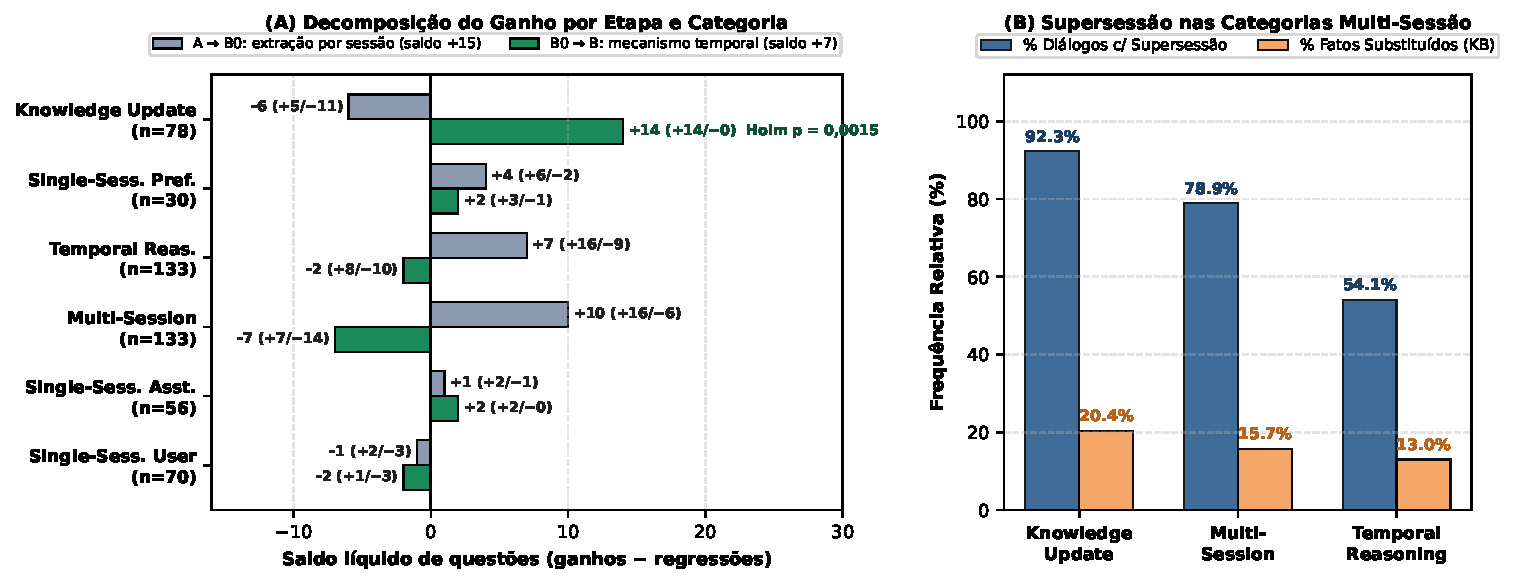
\includegraphics[width=0.95\textwidth]{figures/fig3_analise_pareada_ab.pdf}
\caption{(A) Decomposição do saldo líquido por categoria ($A \rightarrow B_0$ e $B_0 \rightarrow B$). (B) Ativação de supersessões nas categorias multi-sessão da Proposta $B$ \novo{(na variante ontológica $B_{\text{v2}}$, o volume total caiu 53,6\%, de 612 para 284)}.}
\label{fig:analise_pareada}
\end{figure*}

\subsection{\texorpdfstring{\novo{Ablação Fatorial 2$\times$2 (Ranking vs.\ Tags) e Sensibilidade ($\lambda, \tau$)}}{Ablação Fatorial 2x2 (Ranking vs. Tags) e Sensibilidade (lambda, tau)}}
\novo{A Fig.~\ref{fig:ablacao_sens} sintetiza os dois estudos de encerramento realizados sobre os 500 grafos de $B$:}

\begin{figure*}[!t]
\centering
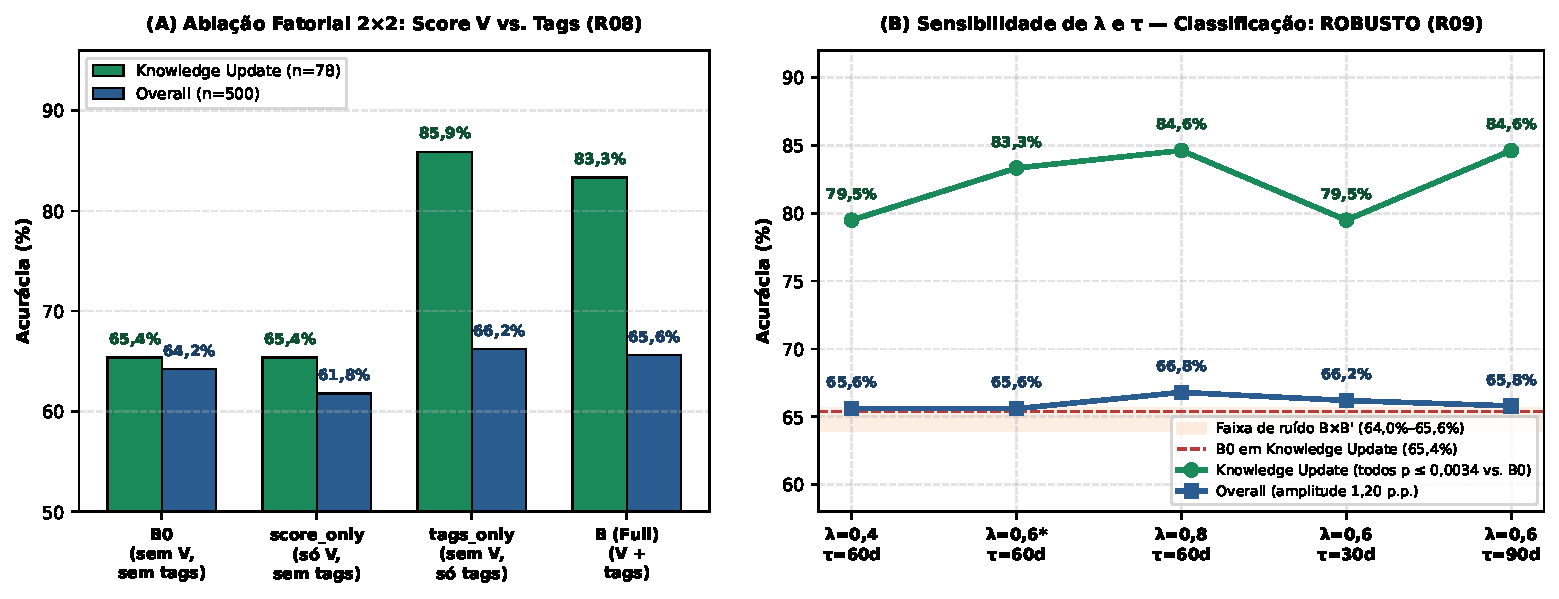
\includegraphics[width=0.96\textwidth]{figures/fig6_ablacao_sensibilidade.pdf}
\caption{\novo{(A) Ablação fatorial 2$\times$2 isolando score $\mathcal{V}$ (\texttt{score\_only}) e etiquetas de vigência (\texttt{tags\_only}) sobre os mesmos 500 grafos. (B) Análise de sensibilidade em $\lambda \in \{0{,}4; 0{,}6; 0{,}8\}$ e $\tau \in \{30, 60, 90\}$ dias (configuração reportada $\lambda=0{,}6, \tau=60$\,d marcada com $*$), confirmando robustez.}}
\label{fig:ablacao_sens}
\end{figure*}

\begin{enumerate}
    \item \novo{\textbf{Tags são o motor causal no recorte \textit{oracle}}: na ablação fatorial (Fig.~\ref{fig:ablacao_sens}A), ativar apenas o score $\mathcal{V}$ sem etiquetas (\texttt{score\_only}) produziu \textbf{efeito nulo em \textit{Knowledge Update}} (51/78, +3/$-$3, $p = 1{,}000$) e queda global para 61,80\%. Como os grafos semânticos possuem em média 9,18 fatos e o \textit{retriever} recupera \texttt{semantic\_top\_k}=5, tanto o fato obsoleto quanto o atual chegam ao prompt; sem etiquetas, a reordenação isolada não resolve o conflito. Já ativar apenas as etiquetas (\texttt{tags\_only}, $\mathcal{V}\equiv 1$) capturou \textbf{100\% do ganho em KU} (\textbf{85,90\%}, +16/$-$0, $p < 0{,}0001$) e atingiu \textbf{66,20\%} no geral. Em bancos maiores com dezenas de sessões distratoras, $\mathcal{V}$ tende a tornar-se necessário como filtro antes do corte \texttt{top-k}.}
    \item \novo{\textbf{Robustez frente a $\lambda$ e $\tau$}: variando $\lambda \in \{0{,}4; 0{,}8\}$ e $\tau \in \{30\text{d}, 90\text{d}\}$ sem seleção de hiperparâmetros no teste (Fig.~\ref{fig:ablacao_sens}B), a acurácia global manteve-se entre \textbf{65,60\% e 66,80\%} (amplitude de 1,20 p.p., inferior ao piso de ruído de 1,60 p.p.; todos $p \ge 0{,}461$ vs.\ $B_{\text{ref}}$) e \textit{Knowledge Update} permaneceu entre \textbf{79,49\% e 84,62\%} (todos $p \le 0{,}0034$ vs.\ $B_0$). O resultado classifica-se como \textbf{ROBUSTO}.}
\end{enumerate}

% =========================================================================
% SEÇÃO V: ANÁLISE QUALITATIVA, AUDITORIA E LIMITAÇÕES
% =========================================================================
\section{Análise Qualitativa, \texorpdfstring{\novo{Auditoria}}{Auditoria} e Limitações}

\begin{figure*}[!t]
\centering
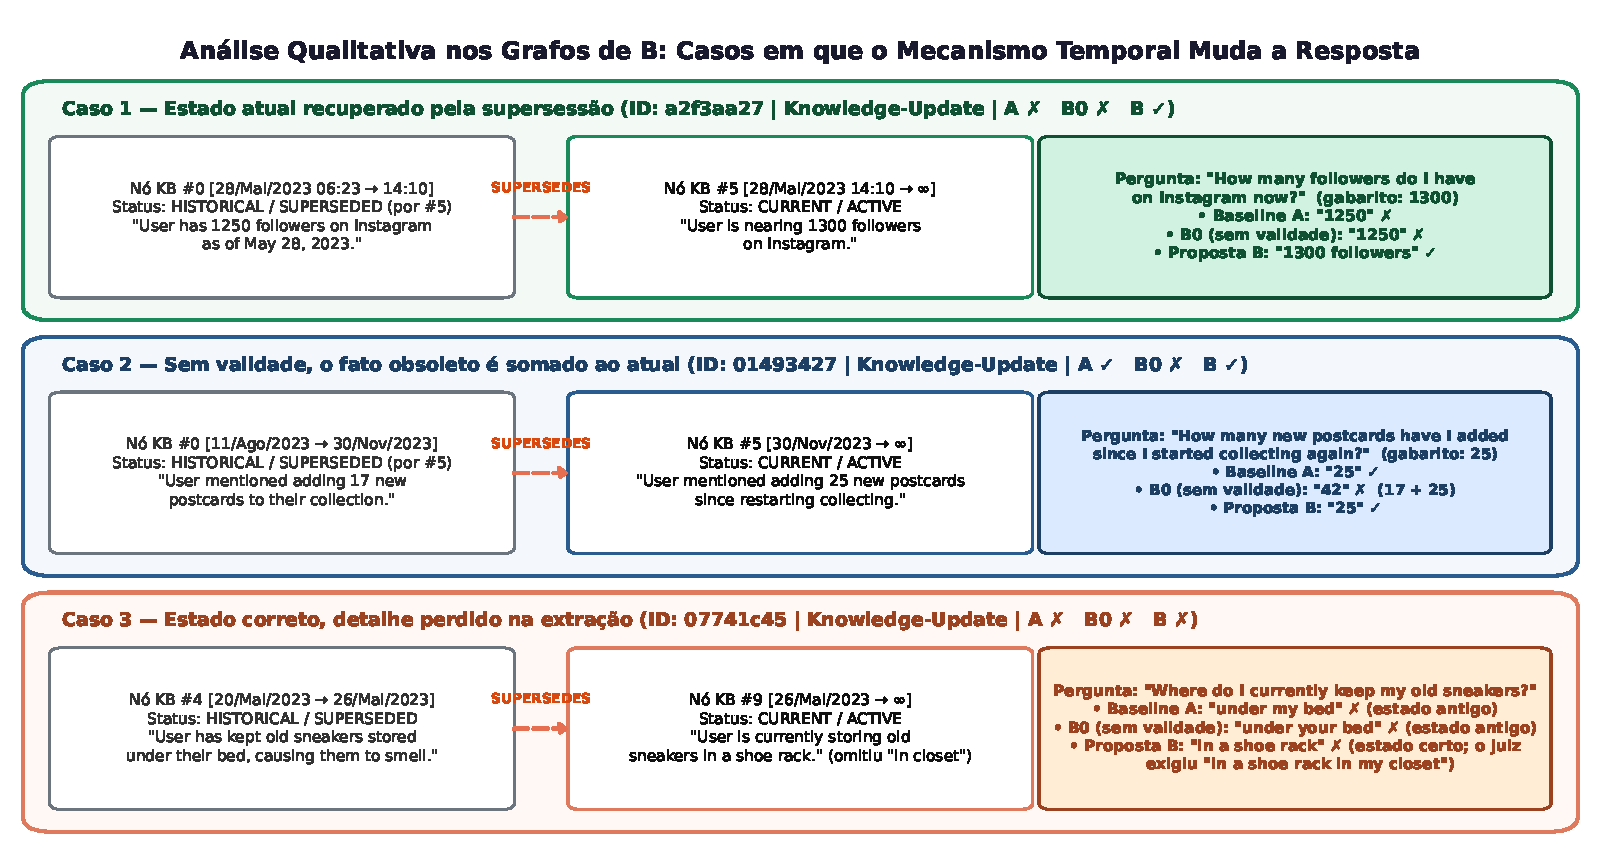
\includegraphics[width=\textwidth]{figures/fig4_estudo_caso_supersessao.pdf}
\caption{Estudos de caso qualitativos nos grafos de $B$: (Caso 1) atualização de estado resolvida apenas pelo mecanismo temporal em \texttt{a2f3aa27}; (Caso 2) interferência factual na $B_0$ somando valor obsoleto ao atual em \texttt{01493427}; (Caso 3) estado corrigido em \texttt{07741c45}, mas penalizado por detalhe perdido na extração.}
\label{fig:estudo_caso}
\end{figure*}

\subsection{Casos Qualitativos \texorpdfstring{\novo{e Auditoria de Precisão da Supersessão}}{e Auditoria de Precisão da Supersessão}}
A Fig.~\ref{fig:estudo_caso} ilustra o mecanismo em operação: em \texttt{a2f3aa27} (seguidores no Instagram: 1.250 $\rightarrow$ 1.300 no mesmo dia), $A$ e $B_0$ respondem o valor obsoleto, enquanto $B$ resolve via etiqueta \texttt{CURRENT}; em \texttt{01493427} (cartões-postais: 17 $\rightarrow$ 25), a $B_0$ soma os dois valores (``42'') por ausência de validade, dano integralmente desfeito por $B$; e em \texttt{07741c45} (localização dos tênis), $B$ corrige o anacronismo mas é penalizada pela compressão lexical do extrator.

\novo{Para quantificar diretamente a \textit{over-supersession}, auditou-se manualmente uma amostra estratificada de 90 transições \texttt{SUPERSEDES} ($n=45$ de $B$ e $n=45$ de $B_{\text{v2}}$, 15 por categoria multi-sessão):}
\begin{itemize}
    \item \novo{\textbf{Salto de precisão em $B_{\text{v2}}$}: a precisão global subiu de \textbf{33,3\%} ($B$) para \textbf{48,9\%} ($B_{\text{v2}}$), com redução de 53,6\% no volume total de arestas. Em \textit{Temporal Reasoning}, a precisão quadruplicou (\textbf{13,3\% $\rightarrow$ 53,3\%}), explicando o recorde de 57,89\% de $B_{\text{v2}}$.}
    \item \novo{\textbf{Gargalo persistente em \textit{Multi-Session}}: a precisão nessa categoria permaneceu baixa (20,0\% em $B$; 26,7\% em $B_{\text{v2}}$), pois eventos ou objetos coexistentes (ex.: \texttt{46a3abf7}, aquário de 5 galões $\rightarrow$ 20 galões; \texttt{gpt4\_2f8be40d}, casamento de amigo $\rightarrow$ próprio casamento) ainda são ocasionalmente marcados como substituição.}
    \item \novo{\textbf{Descoberta estrutural no dataset}: a auditoria revelou que \textbf{34/500 itens} do arquivo distribuído têm \texttt{haystack\_dates} fora de ordem cronológica, produzindo supersessões reversas ($t_{end} < t_{start}$) em 5,6\% das arestas de $B$ (34/612) e 3,2\% de $B_{\text{v2}}$ (9/284) --- \textbf{100\% concentradas em \textit{Temporal Reasoning}}. Ordenar as sessões cronologicamente antes da codificação elimina integralmente essa classe de erro.}
\end{itemize}

\subsection{Limitações e Ameaças à Validade}
\begin{itemize}
    \item \textbf{Recorte \textit{oracle} e dataset único}: avaliou-se o arquivo de 500 questões distribuído com o \textit{HeLa-Mem} (apenas sessões de evidência). A avaliação no \textit{LongMemEval\textsubscript{S}} completo ($\sim$40 sessões/questão) e no \textit{LoCoMo} fica registrada como trabalho futuro.
    \item \textbf{Juiz LLM \novo{e pareamento de grafos episódicos}}: o juiz pertence à mesma família do gerador (\texttt{gpt-4o-mini})\novo{; além disso, $B$, $B_0$ e $B_{\text{v2}}$ reutilizaram os grafos episódicos de $A$ (\texttt{MAX\_FLIPPED}=5, \texttt{KEYWORD\_WEIGHT}=0,5), enquanto $A^*$ usou 3 e 0,7. As comparações internas $B_0 \rightarrow B / B_{\text{v2}} / \texttt{tags\_only}$ são 100\% pareadas sobre os mesmos grafos, e $A^* \rightarrow B_0$ mostrou-se neutra em KU ($p = 0{,}8145$)}.
    \item \novo{\textbf{Sensibilidade de $\theta_{sup}$}: variaram-se $\lambda$ e $\tau$ na etapa de busca; a sensibilidade de $\theta_{sup}=0{,}35$ exige recodificação completa da memória semântica e permanece como limitação.}
\end{itemize}

% =========================================================================
% SEÇÃO VI: CONCLUSÃO
% =========================================================================
\section{Conclusão}
Este trabalho demonstrou, por meio de \novo{reprodução fiel ($A^*$),} ablações controladas ($B_0$\novo{, \texttt{score\_only}, \texttt{tags\_only}}), \novo{quantificação de ruído ($B'$), análise de sensibilidade ($\lambda, \tau$) e auditoria manual de precisão,} que a modelagem explícita de validade temporal e supersessão de fatos é um complemento eficaz \novo{e estatisticamente robusto} para memórias associativas hebbianas em tarefas de atualização de conhecimento (\textit{Knowledge Update}: \novo{+12 acertos sobre $A^*$, $p = 0{,}0042$;} +14/$-$0 sobre $B_0$, $p_{\text{Holm}} = 0{,}0015$). Revelou-se também que (i) fatos semânticos densos sem noção de validade induzem interferência factual, \novo{(ii) no regime \textit{oracle}, a sinalização explícita de vigência no prompt (\texttt{tags\_only}, 85,90\% em KU e 66,20\% global) é o principal vetor causal do ganho,} e (iii) o trade-off em tarefas de agregação decorre de \textit{over-supersession}\novo{, mitigada pela formulação ontológica de \textit{Event Calculus} ($B_{\text{v2}}$)}. Como trabalhos futuros, destacam-se \novo{a ordenação cronológica prévia das sessões (sanando os 34 itens desordenados identificados na auditoria),} a validação no \textit{LongMemEval\textsubscript{S}} completo com distrações \novo{(onde $\mathcal{V}$ atua como filtro de \textit{top-k})} e a extensão para o benchmark \textit{LoCoMo}.

\begin{thebibliography}{00}
\bibitem{helamem2026} R.~Bro et al., ``HeLa-Mem: Hebbian Learning and Associative Memory for LLM Agents,'' in \textit{Proc. ACL}, 2026, pp. 625--639.
\bibitem{zep2025} D.~Chauhan et al., ``Zep: A Temporal Knowledge Graph Architecture for Agent Memory,'' \textit{arXiv:2501.13956}, 2025.
\bibitem{longmemeval2025} D.~Wu et al., ``LongMemEval: Benchmarking Chat Assistants on Long-Term Interactive Memory,'' in \textit{Proc. ICLR}, 2025.
\end{thebibliography}

\end{document}
